\documentclass[oneside]{book}
%\usepackage[margin=.5in]{geometry}

\usepackage{template_professor}


\begin{document}
\begin{multicols}{2}




\subsection{Atividade 1}   Objetivos específicos: Levar o aluno a
\begin{itemize} %s
    \item       Diferenciar a partição da unidade em partes       ``quaisquer''       da partição da unidade em partes       ``iguais''      . A partição em partes iguais será chamada equipartição.
    \item       Reconhecer a necessidade de uma expressão verbal que identifique uma das partes iguais em uma equipartição da unidade.
    \item       Diferenciar       ``a partição da unidade em três partes quaisquer''       da       ``partição da unidade em três partes iguais''      .
    \item       Compreender as expressões ``um terço de'' e ``terça parte de'' como formas de identicar uma das partes da equipartição da unidade em três partes.
\end{itemize} %s



  Recomendações e sugestões para o desenvolvimento da atividade:
\begin{itemize} %s
    \item       Recomenda-se que a atividade seja desenvolvida em grupos de 3 a 5 alunos.
    \item       Busque conduzir a discussão nos grupos de modo que os estudantes percebam que, para que os irmãos recebam a mesma quantidade de chocolate, a partição proposta para a barra de chocolate deve ser em       ``partes iguais''      , no sentido de ganharem todos a mesma quantidade de chocolate, não necessariamente pedaços de mesma forma.
    \item       Na discussão, procure destacar que a referência à       ``partição em três partes iguais''       se dá (igualmente) a partir das expressões       ``um terço''       da barra de chocolate ou       ``a terça parte''       da barra de chocolate.
    \item       O item c) admite diversas soluções, algumas estão apresentadas como resposta. No entanto, algumas dessas respostas podem não aparecer naturalmente em sala de aula. Avalie a possibilidade de apresentar e explorar algumas dessas soluções (ou outras que queira) em sala de aula. Por exemplo, apresente uma dessas divisões aos alunos e peça-os que avaliem a equipartição, explicando sua decisão.
    \item       O item d), provavelmente, pode não ser respondido corretamente pelos alunos. Se for o caso, as expressões ``um terço de'' e ``a terça parte de'' devem ser apresentadas.
    \item       Fique atento às falas dos alunos. Observe que os alunos podem representar e verbalizar as respostas de diferentes modos e que não há uma resposta única para a atividade. Por exemplo, alguns alunos podem precisar de mais tempo do que outros para usar a expressão       ``um terço''       no lugar de       ``partição em três partes iguais''       ou       ``divisão em três partes iguais''      . Ou ainda, observarem que há diferentes representações para a equipartição. Por exemplo,
\end{itemize} %s


\begin{itemize} %s
    \item       Esta atividade pode ser adaptada para alunos com deficiência de visão. Para isso, sugere-se confeccionar os modelos da barra de chocolate  inteira e repartida, que estão disponíveis para reprodução no final do livro, em três materiais diferentes. Por exemplo, papel comum e papéis com texturas diferentes, tecido ou material emborrachado.
\end{itemize} %s

\vfill

\begin{resposta*}{Atividade 1}
  \begin{enumerate}[a),wide,labelindent=0pt] %s
    \item       Este item não possui resposta correta, apenas respostas coerentes com a explicação do aluno. Por exemplo, um estudante pode dizer que sim e explicar que o irmão mais velho deve ficar com uma parte maior porque precisa de mais energia. Mas a resposta esperada é que a divisão não é justa porque as quantidades de chocolate são diferentes. Discuta com os alunos para que entendam a divisão correspondente à resposta esperada.
    \item       Não, eles receberão quantidades diferentes de chocolate, embora cada um receba um único pedaço do chocolate.
    \item       Respostas possíveis:
  \begin{imagem*}[breakable]{}{} - FIGURA ARTÍSTICA - \mbox{} \newline \includegraphics[width=\textwidth, keepaspectratio]{../../livro/media/cap1/secoes/licao1_atv1.png}    \mbox{} \newline      ilustração: Cambrainha   \end{imagem*}
    \item       Cada parte é ``um terço'' da barra ou a ``terça parte'' da barra.
\end{enumerate} %s
\end{resposta*}




\subsection{Atividade 2}

  Objetivos específicos: Levar o aluno a

\begin{itemize} %s
    \item       Perceber que a unidade (no caso, uma pizza) pode ser subdividida em uma quantidade igual de partes sem que essa divisão represente uma equipartição.
    \item       Distinguir uma equipartição dentre partições diversas.
    \item       Diferenciar       ``a divisão da unidade em quatro partes quaisquer''       da       ``divisão da unidade em quatro partes iguais''      .
    \item       Compreender as expressões       ``um quarto de''       e       ``quarta parte de''       como forma de identicar uma das partes da equipartição em 4 partes.
\end{itemize} %s


  Recomendações e sugestões para o desenvolvimento da atividade:

\begin{itemize} %s
    \item       Recomenda-se que a atividade seja desenvolvida em grupos de 3 a 5 alunos.
    \item       As diversas soluções apresentadas pelos diferentes grupos devem ser discutidas com a turma inteira.
    \item       É possível que os alunos utilizem expressões variadas para nomear as partes de pizzas em cada divisão. Por exemplo,       ``a maior quarta parte''      ,       ``a menor quarta parte''      ,       ``as quartas partes iguais entre si''      ,       ``a menor parte''      ,       ``a maior parte''      , dentre outras. É importante que a discussão conduza os alunos ao entendimento de que apenas as partes da equipartição podem ser chamadas de       ``quartos''       da pizza, as demais são simplesmente fatias ou pedaços, por exemplo.
    \item       Os alunos devem reconhecer que apenas uma das repartições propostas sugere a equipartição, respondendo assim a última questão proposta nesta atividade.
    \item       Na ilustração, as crianças dos grupos em que a pizza não está em fatias com iguais quantidades de pizza parecem contrariadas. Recomenda-se levantar a questão:       ``Por que será que elas estão parecendo zangadas?''
    \item       Essa atividade pode ser adaptada para alunos com deficiência visual. Para isso, sugere-se confeccionar os modelos das três pizzas repartidas, que estão disponíveis para reprodução no final do livro, em três materiais diferentes. Por exemplo, papel comum e papéis com texturas diferentes, tecido ou material emborrachado.
\end{itemize} %s


\begin{resposta*}{Atividade 2}
\begin{enumerate} [a),wide,labelindent=0pt] %d
    \item       Sim. Cada grupo repartiu sua pizza em quatro fatias.
    \item       Não, pois algumas fatias têm quantidades de pizza diferentes das outras.
    \item       Apenas no grupo 1 as 4 crianças receberam a mesma quantidade de pizza. Cada fatia da pizza do grupo 1 é       ``um quarto''       da pizza ou       ``a quarta parte''       da pizza. Diferentemente das demais pizzas.
\end{enumerate} %d
\end{resposta*}



\subsection{Atividade 3}
  Objetivo específico:Levar o aluno a
\begin{itemize} %s
    \item       Abordar a equipartição em um modelo linear.
    \item       Reconhecer a quarta parte como a metade da metade.
\end{itemize} %s

  Recomendações e sugestões para o desenvolvimento da atividade:

\begin{itemize} %s
    \item       Recomenda-se que esta atividade seja desenvolvida em grupos de quatro alunos.
    \item       Cada grupo deve receber um pedaço de barbante de, aproximadamente, 1m e quatro enfeites (todos iguais).
    \item       Os quatro enfeites precisam ser confeccionados antes da realização da tarefa. Sugerem-se estrelas, cujos modelos estão disponíveis para reprodução no final do livro. No entanto, segundo a avaliação do professor, os enfeites podem ser outros, desde que sejam os 4 congruentes.
    \item       Como sugestão, se possível, solicitar aos alunos que confeccionem os enfeites, por exemplo, associando esta atividade com geometria, com a abordagem de grandezas e medidas, com a disciplina de artes ou envolvendo culturas artesanais populares.
    \item       A equipartição do barbante não deve ser obtida a partir da medida do barbante, mas por sucessivas dobras do barbante sobre ele mesmo, como ilustrado na resposta da atividade.
    \item       A manipulação e a dobra do barbante devem sustentar a discussão para a identificação da       ``metade da metade''       com a       ``quarta parte''       do barbante. Nesse caso, a identificação se dará pela sobreposição das partes.
\end{itemize} %s


\begin{resposta*}{Atividade 3}

Uma maneira de se cortar o barbante é dobrar ao meio e depois dobrar novamente ao meio, obtendo quatro partes iguais, como ilustrado na figura a seguir.
  \begin{imagem*}[breakable]{}{}     - FIGURA ARTÍSTICA - Sequência de duas imagens que ilustrem um barbante sendo dobrado sobre ele mesmo duas vezes sucessivas, até que se obtenha quartos. Por exemplo, como a imagem a seguir:
        \includegraphics[width=\textwidth, keepaspectratio]{../../livro/media/cap1/secoes/barbante_dobras.jpg}
  \end{imagem*}
\end{resposta*}


\subsection{Sobre o Organizando as Ideias}

  Nesta etapa, espera-se que os alunos compreendam as frações como forma de expressar quantidades. O objetivo é que percebam seu papel para expressar quantidades em situações de equipartição da unidade. Assim, as frações podem ser utilizadas no dia a dia para identificar quantidades do mesmo modo que os números naturais, já conhecidos dos alunos. Por exemplo, como nas expressões:   ``dois ovos''  ,   ``duas xícaras de farinha''  ,   ``um terço de xícara de cacau''   e   ``meio litro de leite''  .

  Objetiva-se a expressão verbal e não a representação simbólica. Espera-se, assim, que os alunos apropriem-se das expressões verbais que identificam as frações unitárias (um meio, um terço, um quarto, ... , um nono e um décimo) antes de serem apresentados formalmente à simbologia matemática (que será objetivo da próxima lição).  A referência às frações unitárias com a expressão   ``um''   antes da identicação da parte, como, por exemplo, em   ``um terço''   e em   ``um sétimo''   é uma decisão pedagógica. Claro que é possível se referir a essas frações simplesmente por   ``terço''   e   ``sétimo''  , respectivamente. No entanto, nas próximas seções, pretende-se que as frações não unitárias, como   ``dois terços''   e   ``nove sétimos''  , por exemplo, sejam entendidas a partir da justaposição das frações unitárias correspondentes, o que é naturalmente amparado pela contagem. Nas expressões verbais relativas às frações unitárias, o   ``um''   antes da identificação da parte está associado à cotagem. Dessa formma, a compreensão das frações   ``um terço''   e   ``dois terços''   ou das frações   ``um sétimo''   e   ``nove sétimos''  , por exemplo, seguem a mesma construção lógica.

\subsection{Atividade 4}
  Objetivo específico: Levar o aluno a:
\begin{itemize} %s
    \item       Reconhecer que, em uma equipartição, as partes podem não ter a mesma forma.
    \item       Identificar a equivalência entre as partes de uma equipartição a partir de sobreposição ou da comparação pelo reconhecimento da associação a uma mesma fração unitária (no caso, $\frac{1}{4}$).
    \item       Reconhecer a quarta parte como a metade da metade.
\end{itemize} %s

  Recomendações e sugestões para o desenvolvimento da atividade:

\begin{itemize} %s
    \item       Recomenda-se que esta atividade seja desenvolvida em grupos de 3 a 5 alunos. Cada grupo deve receber as imagens dos oito retângulos, disponíveis para reprodução no final do livro e colorí-las, cada um com uma cor diferente das demais.
    \item       Em cada grupo, os alunos devem decidir qual (ou quais) das divisões propostas para os retângulos correspondem a uma partição em quartos. É importante observar que todos os retângulos estão divididos em quartos.
    \item       Conduza a discussão de modo a levar os alunos a reconhecer que, em uma equipartição, as partes não precisam ter a mesma forma.
    \item       Se necessário, o professor pode associar cada retângulo a um objeto concreto (por exemplo, uma barra de chocolate ou a um pedaço de bolo). No entanto, nesta atividade, espera-se que os alunos consigam lidar com a figura de um retângulo como representativa de uma unidade genérica.
    \item       Recomenda-se que os alunos recortem as partes de cada um dos retângulos para realizar a comparação por sobreposição. No entanto, essa estratégia não será suficiente para todos os 8 casos. Em alguns casos, a comparação se dará pela identificação da fração unitária correspondente a cada parte. Nesses casos, o aluno deve reconhecer que a quarta parte é equivalente à metade da metade. Por exemplo, como no caso seguir.
\end{itemize} %s

\noindent 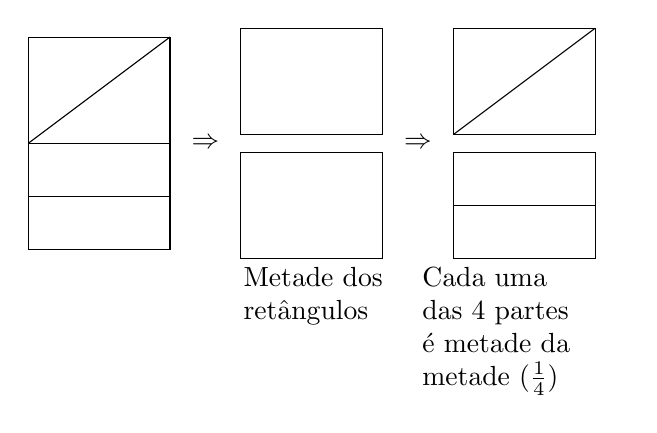
\begin{tikzpicture}[scale=0.45]
  \draw (0,0) rectangle (4,3);
  \draw (0,3) rectangle (4,6);
  \draw (0,1.5) -- (4,1.5);
  \draw (0,3) -- (4,6);
  \draw (5,3) node{$\Rightarrow$};
  \draw (6,-0.25) rectangle (10,2.75);
  \draw (6,3.25) rectangle (10,6.25);
  \node[text width=2cm]  at (8.3,-1.3) { Metade dos retângulos};
  \draw (11,3) node{$\Rightarrow$};
  \draw (12,-0.25) rectangle (16,2.75);
  \draw (12,3.25) rectangle (16,6.25);
  \draw (12,3.25) -- (16,6.25);
  \draw (12,1.25) -- (16,1.25);
  \node[text width=2.5cm]  at (13.9,-2.3) { Cada uma das 4 partes é metade da metade ($\frac{1}{4}$)}; 
  \end{tikzpicture}
\begin{itemize} %s
    \item       Segundo a avaliação do professor, a atividade pode ser realizada em duas etapas. Em um primeiro momento, os alunos recebem as primeiras quatro das oito imagens e realizam a atividade com essas imagens - cuja comparação se dá apenas pela sobreposição. Em seguida, recebem as outras quatro, para concluir a atividade. Para as últimas 4 figuras, será necessário reconhecer a quarta parte como a metade da metade. É importante que o professor, ao final das duas etapas, avalie as escolhas como um todo.
\end{itemize} %s


\begin{resposta*}{Atividade 4}
\begin{enumerate}[a),wide,labelindent=0pt] %s
    \item       Todos os retângulos estão divididos em quartos.
    \item       Dois desenhos possíveis são:
\end{enumerate} %s
\end{resposta*}


\subsection{Atividade 5}
  Objetivo específico: Levar o aluno a:

\begin{itemize} %s
    \item       Identificar uma mesma fração unitária (no caso, a terça parte) em representações diversas, ou seja, em representações de unidades não necessariamente congruentes.
\end{itemize} %s



  Recomendações e sugestões para o desenvolvimento da atividade:
\begin{itemize} %s
    \item       Recomenda-se que esta atividade seja desenvolvida em grupos de 3 a 5 alunos.
    \item       Durante a discussão, os alunos devem ser estimulados a explicar as suas escolhas. A discussão sobre os motivos da identificação, ou não, de cada uma das representações à terça parte da unidade correspondente será fundamental para atingir o objetivo da atividade.
    \item       Os alunos devem reconhecer que, independente da unidade considerada, em uma equipartição em 3 partes, cada uma das partes é um terço (ou a terça parte) da unidade.
    \item       Aproveite as próprias palavras e os argumentos dos alunos para conduzi-los às conclusões esperadas.
    \item       Fique atento aos alunos que selecionarem as figuras que simplesmente possuem alguma associação com o número 3, não correspondendo a terços. Por exemplo, um aluno que associe a       {\bf Figura ZZ}       a terços pode ainda não ter compreendido a necessidade da equipartição para a identificação de um terço. Já o aluno que associa       {\bf Figura ZZ}       a terços pode estar simplesmente contando as partes em vermelho, sem que tenha reconhecido que a figura deveria estar dividida em 3 partes iguais e não em 5.
\end{itemize} %s





\begin{resposta*}{Atividade 5}

A parte em vermelho representa um terço da figura nos itens c), d), e), f) e h).
\end{resposta*}



\subsection{Atividade 6}
  Objetivo específico: Levar o aluno a:
\begin{itemize} %d
    \item       Recompor a unidade a partir de uma fração unitária dada em modelos contínuos.
    \item       Relacionar uma fração da unidade à quantidade necessária dessas partes para compor a unidade. Assim, por exemplo, é necessário reunir cinco       {\it quintas partes}       para recompor o todo.
\end{itemize} %d



  Recomendações e sugestões para o desenvolvimento da atividade:
\begin{itemize} %d
    \item       Recomenda-se que a atividade seja desenvolvida em grupos de 3 a 5 alunos.
    \item       É importante ter em mente que existem várias soluções para cada item. Por exemplo, o primeiro item pode ser corretamente respondido por:             \begin{tikzpicture}[scale=.2]
\draw [fill=common, fill opacity=.3] (0,0) arc (0:180:3) -- (0,0) -- cycle;
\draw (-3,0) -- (-3,3);
\end{tikzpicture}
 e
 \begin{tikzpicture}[scale=.2]
\draw [fill=common, fill opacity=.3] (0,0) arc (0:90:3) -- (-3,0) -- cycle;
\draw [fill=common, fill opacity=.3] (-3,0) arc (270:180:3) -- (-3,3) -- cycle;
\end{tikzpicture}.
    \item       Avalie a possibilidade de discutir com os estudantes respostas que sejam reuniões de partes não justapostas, por exemplo, no primeiro item pode-se ter também             \begin{tikzpicture}[scale=.2]
\draw [fill=common, fill opacity=.3] (0,0) arc (0:90:3) -- (-3,0) -- cycle;
\draw [fill=common, fill opacity=.3] (3.7,0) arc (0:90:3) -- (0.7,0) -- cycle;
\end{tikzpicture}
      como resposta.
    \item       Estimule os alunos a reconhecer (e a fazer) mais do que uma representação para a unidade em cada item.
    \item       Estimule os alunos a, a partir da identificação da fração unitária, determinar a quantidade de partes necessárias para recompor a unidade.
\end{itemize} %d

\begin{resposta*}{Atividade 6}

Algumas possibilidades de respostas para cada linha da tabela do enunciado estão nas respectivas linhas abaixo.

% arcos de círculos 
 \noindent\begin{tabular}{cccc}
 
\begin{tikzpicture}[scale=.2]
\draw [fill=common, fill opacity=.3] (0,0) arc (0:180:3) -- (0,0) -- cycle;
\draw (-3,0) -- (-3,3);
\end{tikzpicture}
&
 
\begin{tikzpicture}[scale=.2]
\draw [fill=common, fill opacity=.3] (0,0) arc (0:90:3) -- (-3,0) -- cycle;
\draw [fill=common, fill opacity=.3] (-3,0) arc (270:180:3) -- (-3,3) -- cycle;
\end{tikzpicture}

&
\begin{tikzpicture}[scale=.2]
\draw [fill=common, fill opacity=.3] (0,0) arc (0:90:3) -- (-3,0) -- cycle;
\draw [fill=common, fill opacity=.3] (3.7,0) arc (0:90:3) -- (0.7,0) -- cycle;
\end{tikzpicture}

\\

\begin{tikzpicture}[scale=.2]
\draw [fill=common, fill opacity=.3] (0,0) arc (0:270:3) -- (-3,0) -- cycle;
\draw (-3,0) -- (-6,0);
\draw (-3,0) -- (-3,3);
\end{tikzpicture}
& 
 
\begin{tikzpicture}[scale=.2]
\draw [fill=common, fill opacity=.3] (0,0) arc (0:90:3) -- (-3,0) -- cycle;
\draw [fill=common, fill opacity=.3] (-3,0) arc (270:180:3) -- (-3,3) -- cycle;
\draw [fill=common, fill opacity=.3] (-3,0) arc (180:270:3) -- (0,0) -- cycle;
\end{tikzpicture}
 &
\begin{tikzpicture}[scale=.2]
\draw [fill=common, fill opacity=.3] (0,0) arc (0:90:3) -- (-3,0) -- cycle;
\draw [fill=common, fill opacity=.3] (3.7,0) arc (0:90:3) -- (0.7,0) -- cycle;
\draw [fill=common, fill opacity=.3] (7.4,0) arc (0:90:3) -- (4.4,0) -- cycle;
\end{tikzpicture}
\\

\begin{tikzpicture}[scale=.2]
\draw [fill=common, fill opacity=.3] (0,0) arc (0:360:3) -- (-3,0) -- cycle;
\draw (-3,0) -- (-6,0);
\draw (-3,0) -- (-3,3);
\draw (-3,0) -- (-3,-3);
\end{tikzpicture}
 &
\begin{tikzpicture}[scale=.2]
\draw [fill=common, fill opacity=.3] (0,3) arc (90:270:3) -- (0,3) -- cycle;
 \draw [fill=common, fill opacity=.3] (3,3) arc (0:-90:3) -- (0,3) -- cycle;
 \draw [fill=common, fill opacity=.3] (0,0) arc (90:0:3) -- (0,-3) -- cycle;
 \draw  (0,0) -- (-3,0);
\end{tikzpicture}
 &
\begin{tikzpicture}[scale=.2]
\draw [fill=common, fill opacity=.3] (0,0) arc (0:90:3) -- (-3,0) -- cycle;
\draw [fill=common, fill opacity=.3] (3.7,0) arc (0:90:3) -- (0.7,0) -- cycle;
\draw [fill=common, fill opacity=.3] (7.4,0) arc (0:90:3) -- (4.4,0) -- cycle;
\draw [fill=common, fill opacity=.3] (11.1,0) arc (0:90:3) -- (8.1,0) -- cycle;
\end{tikzpicture}
 \\
 
\begin{tikzpicture}[scale=.2]
\draw [fill=common, fill opacity=.3] (0,0) rectangle (3,3);
\draw [fill=common, fill opacity=.3] (3,0) rectangle (6,3);
\end{tikzpicture}
 &
\begin{tikzpicture}[scale=.2]
\draw [fill=common, fill opacity=.3] (0,0) rectangle (3,3);
\draw [fill=common, fill opacity=.3] (0,3) rectangle (3,6);
\end{tikzpicture}

&
\begin{tikzpicture}[scale=.2]
\draw [fill=common, fill opacity=.3] (0,0) rectangle (3,3);
\draw [fill=common, fill opacity=.3] (3.7,0) rectangle (6.7,3);
\end{tikzpicture}

\\

\begin{tikzpicture}[scale=.2]
\draw [fill=common, fill opacity=.3] (0,0) rectangle (3,3);
\draw [fill=common, fill opacity=.3] (3,0) rectangle (6,3);
\draw [fill=common, fill opacity=.3] (6,0) rectangle (9,3);
\end{tikzpicture}
 &
\begin{tikzpicture}[scale=.2]
\draw [fill=common, fill opacity=.3] (0,0) rectangle (3,3);
\draw [fill=common, fill opacity=.3] (0,3) rectangle (3,6);
\draw [fill=common, fill opacity=.3] (3,0) rectangle (6,3);
\end{tikzpicture}
 &
 
\begin{tikzpicture}[scale=.2]
\draw [fill=common, fill opacity=.3] (0,0) rectangle (3,3);
\draw [fill=common, fill opacity=.3] (3,3) rectangle (6,6);
\draw [fill=common, fill opacity=.3] (6,0) rectangle (9,3);
\end{tikzpicture}
\\
 
\begin{tikzpicture}[scale=.2]
\draw [fill=common, fill opacity=.3] (0,0) rectangle (3,3);
\draw [fill=common, fill opacity=.3] (3,0) rectangle (6,3);
\draw [fill=common, fill opacity=.3] (6,0) rectangle (9,3);
\draw [fill=common, fill opacity=.3] (9,0) rectangle (12,3);
\end{tikzpicture}
&
\begin{tikzpicture}[scale=.2]
\draw [fill=common, fill opacity=.3] (0,0) rectangle (3,3);
\draw [fill=common, fill opacity=.3] (0,3) rectangle (3,6);
\draw [fill=common, fill opacity=.3] (3,0) rectangle (6,3);
\draw [fill=common, fill opacity=.3] (3,3) rectangle (6,6);
\end{tikzpicture}
&
\begin{tikzpicture}[scale=.2]
\draw [fill=common, fill opacity=.3] (0,3) rectangle (3,6);
\draw [fill=common, fill opacity=.3] (0,0) rectangle (3,3);
\draw [fill=common, fill opacity=.3] (3,0) rectangle (6,3);
\draw [fill=common, fill opacity=.3] (6,0) rectangle (9,3);
\end{tikzpicture}
\\

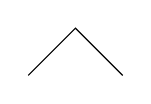
\begin{tikzpicture}[scale=.2]
\draw  (0,0) -- (3,3) -- (6,0);
\end{tikzpicture}
&

\begin{tikzpicture}[scale=.2]
\draw  (0,0) -- (3,3);
\draw  (2,0) -- (5,3);
\end{tikzpicture}
 &

\begin{tikzpicture}[scale=.2]
\draw  (0,0) -- (3,3);
\draw  (3,0) -- (0,3);
\end{tikzpicture}
\\ 

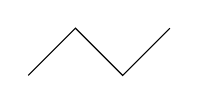
\begin{tikzpicture}[scale=.2]
\draw  (0,0) -- (3,3) -- (6,0) -- (9,3);
\end{tikzpicture}
&

\begin{tikzpicture}[scale=.2]
\draw  (0,0) -- (3,3);
\draw  (2,0) -- (5,3);
\draw  (4,0) -- (7,3);
\end{tikzpicture}
 &

\begin{tikzpicture}[scale=.2]
\draw  (0,0) -- (3,3);
\draw  (4,0) -- (1,3);
\draw  (2,0) -- (5,3);
\end{tikzpicture}
\\ 

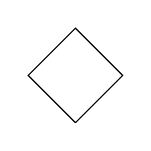
\begin{tikzpicture}[scale=.2]
\draw  (0,0) -- (3,3) -- (0,6) -- (-3,3) -- (0,0);
\end{tikzpicture}
&

\begin{tikzpicture}[scale=.2]
\draw  (0,0) -- (3,3);
\draw  (2,0) -- (5,3);
\draw  (4,0) -- (7,3);
\draw  (6,0) -- (9,3);
\end{tikzpicture}
 &

\begin{tikzpicture}[scale=.2]
\draw  (0,0) -- (3,3);
\draw  (4,0) -- (1,3);
\draw  (2,0) -- (5,3);
\draw (2,0) -- (-1,3);
\end{tikzpicture}
\\

%triängulos
\begin{tikzpicture}[scale=.2]
\draw [fill=common, fill opacity=.3] (0,0) -- (3,0) -- (-1.5,1.5) -- cycle;
\draw [fill=common, fill opacity=.3] (3,0) -- (6,0) -- (1.5,1.5) -- cycle;
\end{tikzpicture}
 
 &
\begin{tikzpicture}[scale=.2]
\draw [fill=common, fill opacity=.3] (0,0) -- (3,0) -- (-1.5,1.5) -- cycle;
\draw [fill=common, fill opacity=.3] (3,0) -- (-1.5,1.5) -- (1.5,1.5) -- cycle;
\end{tikzpicture}
 &
\begin{tikzpicture}[scale=.2]
\draw [fill=common, fill opacity=.3] (0,0) -- (3,0) -- (-1.5,1.5) -- cycle;
\draw [fill=common, fill opacity=.3] (0,0) -- (-1.5,1.5) -- (-4.5,1.5) -- cycle;
\end{tikzpicture}
\\

 
\begin{tikzpicture}[scale=.2]
\draw [fill=common, fill opacity=.3] (0,0) -- (3,0) -- (-1.5,1.5) -- cycle;
\draw [fill=common, fill opacity=.3] (3,0) -- (6,0) -- (1.5,1.5) -- cycle;
\draw [fill=common, fill opacity=.3] (6,0) -- (9,0) -- (4.5,1.5) -- cycle;
\end{tikzpicture}
&
\begin{tikzpicture}[scale=.2]
\draw [fill=common, fill opacity=.3] (0,0) -- (3,0) -- (-1.5,1.5) -- cycle;
\draw [fill=common, fill opacity=.3] (3,0) -- (-1.5,1.5) -- (1.5,1.5) -- cycle;
\draw [fill=common, fill opacity=.3] (-1.5,1.5) -- (1.5,1.5) -- (-3,3) -- cycle;
%\draw [fill=common, fill opacity=.3] (1.5,1.5) -- (-3,3) -- (0,3) -- cycle;
\end{tikzpicture}
 &
\begin{tikzpicture}[scale=.2]
\draw [fill=common, fill opacity=.3] (0,0) -- (3,0) -- (-1.5,1.5) -- cycle;
\draw [fill=common, fill opacity=.3] (0,0) -- (-1.5,1.5) -- (-4.5,1.5) -- cycle;
\draw [fill=common, fill opacity=.3] (-3,0) -- (0,0) -- (-4.5,1.5) -- cycle;
\end{tikzpicture}
\\

\begin{tikzpicture}[scale=.2]
\draw [fill=common, fill opacity=.3] (0,0) -- (3,0) -- (-1.5,1.5) -- cycle;
\draw [fill=common, fill opacity=.3] (3,0) -- (6,0) -- (1.5,1.5) -- cycle;
\draw [fill=common, fill opacity=.3] (6,0) -- (9,0) -- (4.5,1.5) -- cycle;
\draw [fill=common, fill opacity=.3] (9,0) -- (12,0) -- (7.5,1.5) -- cycle;
\end{tikzpicture}
 &
 
\begin{tikzpicture}[scale=.2]
\draw [fill=common, fill opacity=.3] (0,0) -- (3,0) -- (-1.5,1.5) -- cycle;
\draw [fill=common, fill opacity=.3] (3,0) -- (-1.5,1.5) -- (1.5,1.5) -- cycle;
\draw [fill=common, fill opacity=.3] (-1.5,1.5) -- (1.5,1.5) -- (-3,3) -- cycle;
\draw [fill=common, fill opacity=.3] (1.5,1.5) -- (-3,3) -- (0,3) -- cycle;
\end{tikzpicture}
 &
\begin{tikzpicture}[scale=.2]
\draw [fill=common, fill opacity=.3] (0,0) -- (3,0) -- (-1.5,1.5) -- cycle;
\draw [fill=common, fill opacity=.3] (0,0) -- (-1.5,1.5) -- (-4.5,1.5) -- cycle;
\draw [fill=common, fill opacity=.3] (-3,0) -- (0,0) -- (-4.5,1.5) -- cycle;
\draw [fill=common, fill opacity=.3] (-4.5,1.5) -- (-1.5,1.5) -- (-6,3) -- cycle;
\end{tikzpicture}\\

\end{tabular}

\end{resposta*}



\subsection{Atividade 7}

  Objetivos específicos: Levar o aluno a:
\begin{itemize} %s
    \item       Representar uma fração unitária a partir de uma unidade dada.
    \item       Reconhecer (e obter) um quarto como a metade da metade e um oitavo como a metade de um quarto.
    \item       Comparar as frações unitárias metade, um quarto e um oitavo de um mesmo quadrado.
\end{itemize} %s


  Recomendações e sugestões para o desenvolvimento da atividade:
\begin{itemize} %s
    \item       Esta é uma atividade que o aluno pode fazer individualmente.
    \item       Não se espera que, nesta atividade, os alunos usem a medida para fazer a equipartição de maneira mais precisa. O objetivo é fazer a equipartição livremente e de forma coerente. Assim, por exemplo, podem ser aceitas como respostas:
\end{itemize} %s

\begin{tikzpicture}
 \draw[fill=common, fill opacity=.3] (0,0) rectangle (3,3);
 \draw[decorate, decoration={snake, amplitude= .2 mm}] (1.5,0) -- (1.5,3);
\end{tikzpicture} 
e
\begin{tikzpicture}
 \draw[fill=common, fill opacity=.3] (0,0) rectangle (3,3);
 \draw[decorate, decoration={snake, amplitude= .2 mm}] (0,0) -- (3,3);
\end{tikzpicture}

  Já as representações a seguir sugerem que os alunos precisam revisar os conceitos exigidos para a solução da atividade:

  \begin{tikzpicture}
 \draw[fill=common, fill opacity=.3] (0,0) rectangle (3,3);
 \draw[decorate, decoration={snake, amplitude= .2 mm}] (2.3,0) -- (2.3,3);
\end{tikzpicture}

\begin{itemize} %s
    \item       A representação da unidade se dá de forma genérica por um quadrado.
    \item       Espera-se que os alunos reconheçam que para obter um quarto da unidade basta tomar a metade da metade. E que, para determinar um oitavo pode dividir um quarto ao meio.
    \item       Recomende que os alunos usem dobradura para identificar as frações pedidas. Assim, por exemplo, a fração       $\frac{1}{4}$       pode ser obtida por duas dobras do papel.
    \item       Discuta com os estudantes que quanto maior o número de partes iguais em que se particiona o quadrado, menor fica cada uma das partes.
    \item       Procure apresentar e discutir com a turma mais do que uma solução para cada item.
    \item             {\bf As diferentes soluções apresentadas pelos alunos podem enriquecer a discussão}      . A comparação entre, por exemplo, a metade do quadrado proveniente da dobradura pela diagonal e o quarto do quadrado proveniente da dobradura a partir de linhas paralelas aos lados (como um sinal de       ``$+$''      ) pode não ser tão natural. Dificuldade semelhante pode ser observada na comparação entre esse mesmo quarto do quadrado e o oitavo do quadrado proveniente de uma sequência de dobraduras paralelas a um dos lados, determinando       ``faixas paralelas''      . Nesses casos, para executar a comparação, é necessário que os alunos reconheçam partes de formatos diferentes que correspondem a uma mesma fração do quadrado como iguais em quantidade. Assim, a comparação entre a metade do quadrado, obtida pela dobradura na diagonal, e o quarto do quadrado, obtido pela dobraduta       ``em sinal de $+$''      , pode ser amparada pelo reconhecimento de que a metade em questão é igual em quantidade à metade do quadrado obtida por uma única dobra paralela a um dos lados, que é o dobro do quarto do quadrado.
\end{itemize} %s

\begin{resposta*}{Atividade 7}

  Algumas soluções possíveis, convencionais e outras menos convencionais são:

        \begin{enumerate}[a)]
         \item Metade:   \newline    
        \begin{tikzpicture}[scale=.8]	
         \draw[fill=common, fill opacity=.3] (0,0) rectangle (2,2);
         \draw[fill=attention] (0,1) rectangle (2,2);
        \end{tikzpicture}
        \begin{tikzpicture}[scale=.8]	
         \draw[fill=common, fill opacity=.3] (0,0) rectangle (2,2);
         \draw[fill=attention] (0,0) -- (2,2) -- (0,2)--cycle;
        \end{tikzpicture}
        \begin{tikzpicture}[scale=.8]	
         \draw[fill=common, fill opacity=.3] (0,0) rectangle (2,2);
         \draw[fill=attention] (0,2) -- (2,2) -- (1,1)--cycle;
         \draw[fill=attention] (0,0) -- (2,0) -- (1,1)--cycle;
        \end{tikzpicture}
        \begin{tikzpicture}[scale=.8]	
         \draw[fill=common, fill opacity=.3] (0,0) rectangle (2,2);
         \draw[fill=attention] (0,1) rectangle (1,2);
         \draw[fill=attention] (1,0) rectangle (2,1);
        \end{tikzpicture}
       \item Um quarto:  \newline        
       \begin{tikzpicture}[scale=.8]	
         \draw[fill=common, fill opacity=.3] (0,0) rectangle (2,2);
         \draw[fill=attention] (0,0) rectangle (.5,2);
       \end{tikzpicture}
       \begin{tikzpicture}[scale=.8]	
         \draw[fill=common, fill opacity=.3] (0,0) rectangle (2,2);
         \draw[fill=attention] (0,1) rectangle (1,2);
         \draw (1,0) -- (1,1);
         \draw (1,1)-- (2,1);
        \end{tikzpicture}
        \begin{tikzpicture}[scale=.8]	
         \draw[fill=common, fill opacity=.3] (0,0) rectangle (2,2);
         \draw[fill=attention] (0,0) -- (1,1) -- (0,2)--cycle;
         \draw (1,1) -- (2,2);
         \draw (1,1) -- (2,0);
        \end{tikzpicture}
        \begin{tikzpicture}[scale=.8]	
         \draw[fill=common, fill opacity=.3] (0,0) rectangle (2,2);
         \draw[fill=attention] (2,2) -- (1,2) -- (1,1)--cycle;
         \draw[fill=attention] (0,0) -- (1,0) -- (1,1)--cycle;
         \draw (0,2) -- (2,0);
        \end{tikzpicture}
       \item  Um oitavo:  \newline 
       \begin{tikzpicture}[scale=.8]	
         \draw[fill=common, fill opacity=.3] (0,0) rectangle (2,2);
         \draw[fill=attention] (0,0) rectangle (.25,2);
         \foreach \x in {.5,.75,...,1.75} \draw (\x,0) -- (\x, 2);
       \end{tikzpicture}
       \begin{tikzpicture}[scale=.8]	
         \draw[fill=common, fill opacity=.3] (0,0) rectangle (2,2);
         \draw[fill=attention] (0,1) rectangle (.5,2);
         \draw (0,1)--(2,1);
         \foreach \x in {.5,1,...,1.5} \draw (\x,0) -- (\x,2);
        \end{tikzpicture}
        \begin{tikzpicture}[scale=.8]	
         \draw[fill=common, fill opacity=.3] (0,0) rectangle (2,2);
         \draw[fill=attention] (0,1) -- (1,1) -- (0,2)--cycle;
         \draw (0,0) -- (1,1);
        \end{tikzpicture}
        \begin{tikzpicture}[scale=.8]	
         \draw[fill=common, fill opacity=.3] (0,0) rectangle (2,2);
         \draw[fill=attention] (2,2) -- (1,2) -- (1,1)--cycle;
         \draw (1,1) -- (1,0);
         \draw (0,0) -- (1,1);
         \end{tikzpicture}
       \item  Dentre as opções apresentadas, a maior fração do quadrado é metade.
        \end{enumerate}
\end{resposta*}

\subsection{Atividade 8}

  Objetivos específicos: Levar o aluno a:
\begin{itemize} %s
    \item       Representar uma fração unitária (no caso, um meio ou metade) a partir de uma unidade dada.
    \item       Estabelecer representações diferentes para a mesma fração unitária e para uma mesma unidade.
\end{itemize} %s


  Recomendações e sugestões para o desenvolvimento da atividade:
\begin{itemize} %s
    \item       Essa é uma atividade que o aluno pode fazer individualmente.
    \item       Como na atividade anterior, não se espera que, nesta atividade, o aluno use a medida para fazer a equipartição de maneira mais precisa. O objetivo é que o aluno faça a equipartição livremente e de forma coerente.
    \item       Incentive os alunos a usar dobradura para decidir sobre as diferentes formas de identificar metades na unidade apresentada.
\end{itemize} %s

Observe que a representação da unidade se dá de forma genérica, ainda em modelo contínuo, por uma figura não tradicional como retângulos e círculos, que é determinada pela justaposição de dois hexágonos regulares.

\begin{itemize} %s
    \item       Procure apresentar e discutir com a turma mais do que uma solução para cada item.
\end{itemize} %s

\begin{resposta*}{Atividade 8}

Algumas das respostas possíveis para este problema são:
\begin{center}
\begin{tikzpicture}[scale=.4]
\draw[fill=attention] (3.,5.) -- (3.,3.) -- (4.7,2.) -- (6.46,3.) -- (6.46,5.) -- (4.73,6.) -- cycle;
\draw[fill=common, fill opacity=.3] (6.46,5.) -- (6.46,3.) -- (8.2,2.) -- (9.9,3.) -- (9.9,5.) -- (8.2,6.) -- cycle;
\end{tikzpicture}
\begin{tikzpicture}[scale=.4]
\draw[fill=common, fill opacity=.3] (3.,5.) -- (3.,3.) -- (4.7,2.) -- (6.46,3.) -- (6.46,5.) -- (4.73,6.) -- cycle;
\draw[fill=common, fill opacity=.3] (6.46,5.) -- (6.46,3.) -- (8.2,2.) -- (9.9,3.) -- (9.9,5.) -- (8.2,6.) -- cycle;
\draw[fill=attention] (4.732050807568877,6.) -- (3.,5.) -- (3.,3.) -- (4.732050807568877,2.) -- cycle;
\draw[fill=attention] (8.2,6.) -- (8.2,2.) -- (9.9,3.) -- (9.9,5.) -- cycle;
\end{tikzpicture}

\begin{tikzpicture}[scale=.4]
\draw[fill=common, fill opacity=.3] (3.,5.) -- (3.,3.) -- (4.7,2.) -- (6.46,3.) -- (6.46,5.) -- (4.73,6.) -- cycle;
\draw[fill=common, fill opacity=.3] (6.46,5.) -- (6.46,3.) -- (8.2,2.) -- (9.9,3.) -- (9.9,5.) -- (8.2,6.) -- cycle;
\draw[fill=attention] (3.,4.) -- (3.,3.) -- (4.732050807568877,2.) -- (6.464101615137757,3.) -- (8.196152422706634,2.) -- (9.928203230275509,3.) -- (9.928203230275509,4.) -- cycle;
\end{tikzpicture}
\begin{tikzpicture}[scale=.4]
\draw[fill=common, fill opacity=.3] (3.,5.) -- (3.,3.) -- (4.7,2.) -- (6.46,3.) -- (6.46,5.) -- (4.73,6.) -- cycle;
\draw[fill=common, fill opacity=.3] (6.46,5.) -- (6.46,3.) -- (8.2,2.) -- (9.9,3.) -- (9.9,5.) -- (8.2,6.) -- cycle;
\draw[fill=attention] (3,5) -- (3.,3.) -- (4.73,2.) -- (6.46,3.) -- (8.2,2.) -- (9.9,3.) -- cycle;
\end{tikzpicture}
\end{center}
\end{resposta*}




\subsection{Atividade 9}
  Objetivos específicos: Levar o aluno a:
\begin{itemize} %s
    \item       Reconhecer a metade de uma unidade pela reunião de partes menores e em partições diversas.
    \item       Estabelecer representações diferentes para a mesma fração unitária para uma mesma unidade.
\end{itemize} %s


  Recomendações e sugestões para o desenvolvimento da atividade:
\begin{itemize} %s
    \item       Esta é uma atividade que o aluno pode fazer individualmente.
    \item       Esta atividade pretende levar o aluno a perceber que a metade de uma unidade pode ser considerada e identificada mesmo sem que se tenha uma divisão em duas partes iguais.
    \item       Como nas atividades anteriores, não se espera que o aluno use a medida para confirmar a metade da unidade. O objetivo é que o aluno identifique a representação da metade (ou não) por sobreposição e justaposição das partes, decompondo e recompondo a figura.
    \item       Cada aluno deve receber as imagens das figuras, disponíveis para reprodução no final do livro para que possa manipular como achar melhor e conduzir a sua decisão.
    \item       Incentive os alunos a argumentar, justificando a sua decisão. Para isso, podem, por exemplo, se apoiar em dobraduras ou no recorte das partes da figura.
    \item       Procure apresentar e discutir com a turma mais do que uma solução para cada item.
\end{itemize} %s





\begin{resposta*}{Atividade 9}

  As figuras que correspondem à metade da unidade são as de números 1, 2, 4, 5, 6, 8, 9, 11 e 12.
\end{resposta*}

\subsection{Atividade 10}



Objetivos específicos: Levar o aluno a:
\begin{itemize}
 \item Distinguir frações unitárias a partir de representações em modelos de área circular.
\item     Comparar frações unitárias a partir de representações em modelos de área circular.
\end{itemize}

    
Recomendações e sugestões para o desenvolvimento da atividade:
\begin{itemize}
 \item Recomenda-se que esta atividade seja desenvolvida em grupos de 3 a 5 alunos. No entanto, cada aluno deve ter o seu próprio material (Círculos de Frações) para realizar a atividade.
 \item   Durante a discussão, os alunos devem ser estimulados a explicar as suas escolhas. A discussão sobre os motivos da identificação, ou não, de cada uma das representações às frações da unidade correspondentes será fundamental para atingir o objetivo da atividade.
 \item    Esta atividade é planejada para ser desenvolvida a partir material concreto baseado em modelos de área circular. Mais especificamente com um material conhecido como ``Círculos de Frações''. Para aplicá-la, é necessário reproduzir esse material, que está disponível nas páginas para reprodução.
    \item Sendo um material concreto, os círculos de frações têm o papel de auxiliar na visualização da representação das frações, mais especificamente, das frações unitárias.
    \item Na versão utilizada nesta atividade, o círculo corresponde à unidade, ou seja, ao 1 e os setores circulares, diferenciados por cores, correspondem às frações unitárias um meio, um terço, um quarto, um sexto, um sétimo, um oitavo, um nono e um décimo.
    \item Os Círculos de Frações também podem ser utilizados para tratar das frações unitárias, bem como para a abordagem de outros conceitos e assuntos como, por exemplo, frações em geral, comparação de frações ou as operações de adição e de subtração com frações.
    \item Refira-se ao círculo inteiro (na cor preta) como círculo ou unidade, e não como todo. Refira-se a cada setor circular como fração do círculo, parte do círculo ou, simplesmente, peça da cor x.
    \item Antes de pedir que os alunos façam a atividade, explore o material ressaltando especialmente o fato de que, reunidas, as peças de uma mesma cor determinam um círculo congruente ao preto.
    \item Ainda antes de pedir que os alunos façam a atividade, explore também o material com perguntas dirigidas a toda a turma como as seguintes: ``Quantas peças azuis cobrem o círculo preto?'' ou ``Quantas peças verdes cobrem o círculo preto?''.
    \item Use o material concreto para ilustrar e explicar a resposta de cada item e incentive os seus alunos a fazerem o mesmo.
    \item Espera-se que a explicação para as respostas, nos oito primeiros itens desta questão, seja a partir da contagem dos setores circulares correspondentes às frações envolvidas. Assim, por exemplo, a resposta do item b) pode ser justificada pelo fato de que são necessários 4 partes de círculo na cor vermelha para compor um círculo preto.
    \item Já para os cinco itens que tratam da comparação, espera-se que os alunos identifiquem os setores que representam as fraçoes envolvidas e procedam a comparação pela sobreposição das peças correspondentes. Assim, por exemplo, a resposta do item l) pode ser justificada pela sobreposição das peças das cores verde e amarelo.
    \item Aproveite a correção desses últimos itens para explorar, a partir dos círculos de Frações, a relação entre a quantidade de peças de cada cor e o tamanho das peças, ou seja, a relação inversa entre a quantidade de partes em que círculo (unidade) está dividido e o tamanho de cada parte.
\end{itemize}


\begin{resposta*}{Atividade 10}
\begin{enumerate}[a)]
 \item Uma peça da cor AZUL é igual a um terço do círculo preto.
 \item    Uma peça da cor VERMELHO é igual a um quarto do círculo preto.
 \item    Uma peça da cor AMARELO é igual a um sétimo do círculo preto.
 \item    Uma peça da cor LARANJA é igual a um nono do círculo preto.
 \item    Uma peça da cor roxa é igual a UM SEXTO do círculo preto.
 \item    Uma peça da cor cinza é igual a UM OITAVO do círculo preto.
 \item    Uma peça da cor branca é igual a UM DÉCIMO do círculo preto.
 \item    Uma peça da cor rosa é igual à METADE do círculo preto.
 \item    Um terço do círculo preto é maior do que um sétimo do círculo preto.
 \item    Um nono do círculo preto é menor do que um quarto do círculo preto.
 \item    Um sétimo do círculo preto é menor quinto do círculo preto.
 \item    Um quarto do círculo preto é maior do que um oitavo do círculo preto.
 \item    Um sexto do círculo preto é maior do que um sétimo do círculo preto
\end{enumerate}

\end{resposta*}


\subsection{Atividade 11}
  Objetivos específicos: Levar o aluno a
\begin{itemize} %s
    \item       Conhecer e compreender as expressões correspondentes as frações unitárias com denominadores de 5 a 10.
    \item       Comparar frações da unidade através da representação visual de frações do círculo.
\end{itemize} %s


  Recomendações e sugestões para o desenvolvimento da atividade:
\begin{itemize} %s
    \item       Esta atividade pode ser resolvida individualmente, mas é essencial que seja discutida com toda a turma.
    \item       É provável que nem todos os alunos conheçam ou intuam as expressões correspondentes às frações propostas. Nesse caso, cabe ao professor apresentá-las e diferenciá-las.
    \item       Aproveite esta atividade para revisar e discutir o vocabulário que é objetivo nesta seção:       {\it unidade,}             {\it metade,}             {\it um meio,}             {\it um terço,}             {\it terça parte,}             {\it um quarto,}             {\it quarta parte,}             {\it um quinto,}             {\it quinta parte,}             {\it um sexto,}             {\it sexta parte,}             {\it um sétimo,}             {\it sétima parte,}             {\it um oitavo,}             {\it oitava parte,}             {\it um nono,}             {\it nona parte,}             {\it um décimo}       e       {\it décima parte}      .
\end{itemize} %s




\begin{resposta*}{Atividade 11}
\begin{enumerate}[a),wide,labelindent=0pt] %s
    \item       A correspondência adequada é:
\begin{enumerate} [\;\; I), labelindent=0pt] %d
        \item           A esta afirmação corresponde a figura G).
        \item           A esta afirmação corresponde a figura D).
        \item           A esta afirmação corresponde a figura I).
        \item           A esta afirmação corresponde a figura B).
        \item           A esta afirmação corresponde a figura A).
        \item           A esta afirmação corresponde a figura F).
\end{enumerate} %d

    \item       As frações um sétimo, um oitavo, um nono e um décimo do círculo são menores que um sexto do círculo. Qualquer uma delas está correta.
    \item       As frações um meio, um terço, um quarto, um quinto, um sexto, um sétimo e um oitavo do círculo são maiores que um nono do círculo. Qualquer uma delas está correta.
    \item       As frações um sétimo e um oitavo do círculo são menores que um sexto e maiores que um nono do círculo.
\end{enumerate} %s
\end{resposta*}




\subsection{Atividade 12}

  Objetivos específicos: Levar o aluno a:
\begin{itemize} %s
    \item       Distinguir frações unitárias a partir de representações em modelos diversos, baseados em equipatição ou não.
    \item       Comparar frações unitárias a partir de representações em modelos diversos, baseados em equipatição ou não.
    \item       Estabelecer a comparação entre as frações       ``um meio''      ,       ``um quarto''       e       ``um décimo''      .
    \item       Reconhecer e diferenciar a representação das frações       ``um meio''      ,       ``um quarto''       e       ``um décimo''       em modelos diversos, baseados em equipatição ou não.
    \item       Estabelecer a comparação entre as frações       ``um meio''      ,       ``um quarto''       e       ``um décimo''
\end{itemize} %s


  Recomendações e sugestões para o desenvolvimento da atividade:
\begin{itemize} %s
    \item       Esta é uma atividade que o aluno pode fazer individualmente.
    \item       Esta atividade pretende levar o aluno a perceber que a metade de uma unidade pode ser considerada e identificada mesmo sem que se tenha uma divisão em duas partes iguais.
    \item       Como nas atividades anteriores, não se espera que os alunos usem a medida para confirmar a metade. O objetivo é que identifiquem a representação da metade (ou não) por sobreposição e justaposição dasa partes, decompondo e recompondo a figura.
    \item       Cada aluno deve receber as imagens das figuras, disponíveis para reprodução no final do livro para que possa manipular como achar melhor e conduzir a sua decisão.
    \item       Incentive os alunos a argumentar, justificando a sua decisão. Para isso, podem, por exemplo, se apoiar em dobraduras ou no recorte das partes da figura.
    \item       Procure apresentar e discutir com a turma mais do que uma solução para cada item
\end{itemize} %s


\begin{resposta*}{Atividade 12}

\noindent
(A) um meio,  (B) um décimo, (C) um quarto,\\
(D) um quarto, (E) um quarto, (F) um meio,\\
(G) um quarto, (H) um décimo, (I) um quarto,\\
(J) um décimo, (L) um quarto, (M) um meio
\end{resposta*}



\end{multicols}

\end{document}